\documentclass[paper=a4, fontsize=11pt]{scrartcl} % A4 paper and 11pt font size
\usepackage{./../usfassignment}
\settitle{Assignment 10}
\setauthor{Wanzhang Sheng}
\setcourse{CS675: Automata Theory}

\begin{document}

\maketitle % Print the title

% -----------------------------------------------------------------------------
% PROBLEM 1
% -----------------------------------------------------------------------------
\section{}

\begin{fancyquotes}
  (8 points) Give a Turing Machine for the language $L=\{a^ib^j:i<j\}$
\end{fancyquotes}

\begin{figure}[hp]
  \centering
  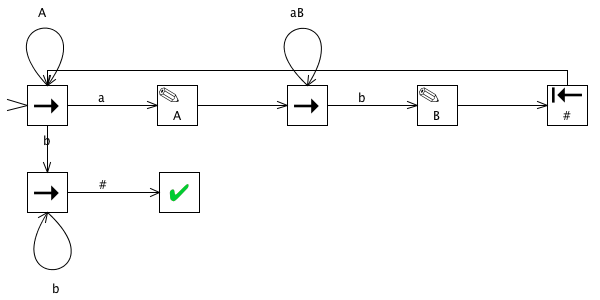
\includegraphics[width=\textwidth]{10-1.png}
\end{figure}

\pagebreak

% -----------------------------------------------------------------------------
% PROBLEM 2
% -----------------------------------------------------------------------------
\section{}

\begin{fancyquotes}
   (8 points) Give a Turing Machine that computes the function $f(x) =
   2x + 2$, where $x$ is in binary. You can assume that the tape
   starts our as $\rhd\underline{\sqcup}w$, and the machine should end
   with the tape in the configruation $\rhd\underline{\sqcup}v$ (where
   $v$ is the binary representation of $2\times w + 2$). You can
   assume that all inputs will be valid numbers $>0$, and leading
   zeroes in your output are acceptable.
\end{fancyquotes}

\begin{figure}[hp]
  \centering
  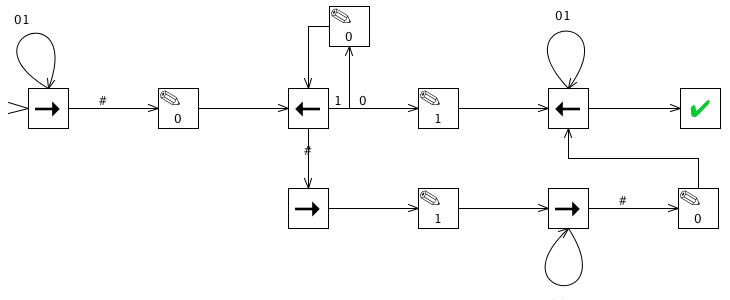
\includegraphics[width=\textwidth]{10-2.png}
\end{figure}

\pagebreak

% -----------------------------------------------------------------------------
% PROBLEM 3
% -----------------------------------------------------------------------------
\section{}

\begin{fancyquotes}
  (8 points) Give a non-deterministic machine (For each string in the
  language, there is some computational path that halts and says
  ``yes'', and perhaps some computational paths that halt and say
  ``no''), that decides the language $L=\{www: w\in\{a,b\}^*\}$
\end{fancyquotes}

\begin{figure}[hp]
  \centering
  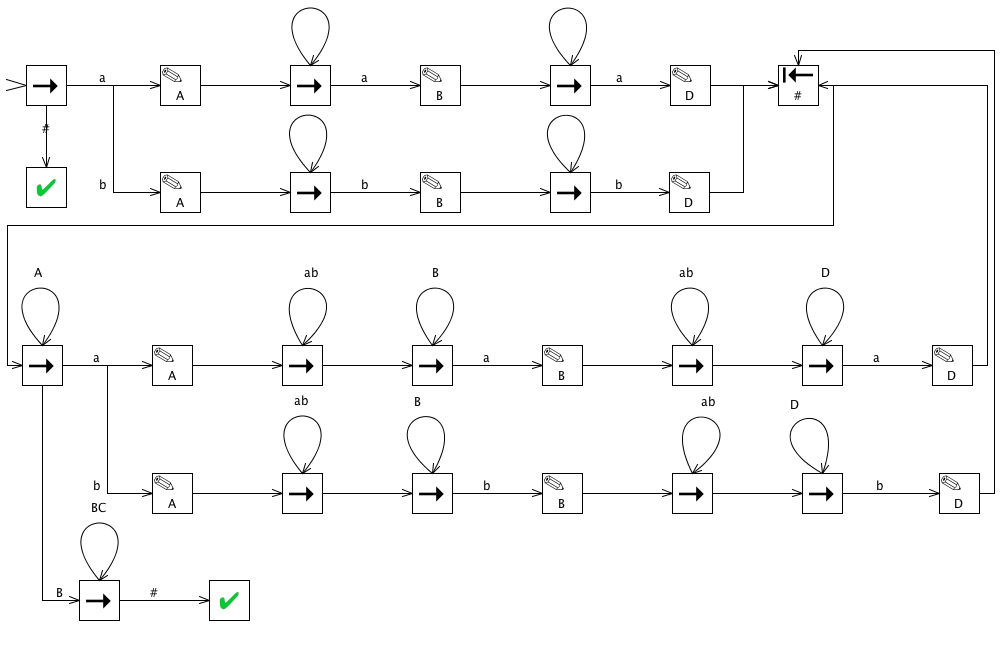
\includegraphics[width=\textwidth]{10-3.png}
\end{figure}

\pagebreak

% -----------------------------------------------------------------------------
% PROBLEM 4
% -----------------------------------------------------------------------------
\section{}

\begin{fancyquotes}
  (8 points) Give a 1-Counter machine that accepts the following
  language: $L = \{a^nba^{2n} : n\geq 1\}$. Thus $abaa, aabaaaa,
  aaabaaaaaa, aaaabaaaaaaaa \in L$, while $abbaa, aba, aaa \in L$.
\end{fancyquotes}

\begin{figure}[hp]
  \centering
  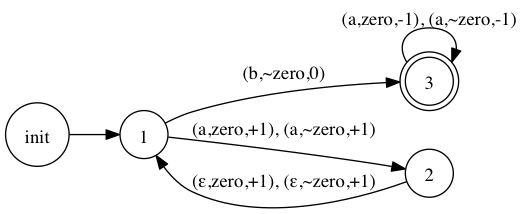
\includegraphics[width=\textwidth]{10-4.gv.png}
\end{figure}

\pagebreak

\end{document}